%%%%%%%%%%%%%%%%%%%%%%%%%%%%%%%%%%%%%%%%%%%%%%%%%%%%%%%%%%%%%%%%%%%%%%%%%%%%%%%%%%
%%																				%%
%% File name: 		20hannes.tex												%%
%% Project name:	Hochleistungsantenne										%%
%% Type of work:	T3X00 project work											%%
%% Author:			Sarah Brückner, Maximilian Stiefel, Hannes Bohnengel		%%
%% Date:			31th May 2016												%%
%% University:		DHBW Ravensburg Campus Friedrichshafen						%%
%% Comments:		Created in gedit with tab width = 4							%%
%%																				%%
%%%%%%%%%%%%%%%%%%%%%%%%%%%%%%%%%%%%%%%%%%%%%%%%%%%%%%%%%%%%%%%%%%%%%%%%%%%%%%%%%%

\chapter{Aufbau der Bodenstation}

Die Bodenstation der DHBW Ravensburg am Standort Friedrichshafen besteht grundsätzlich aus folgenden Komponenten:

\begin{itemize}
	\parskip0pt
	\item Antennen (drei Bänder)
	\begin{itemize}
		\item Endstufen / Verstärker
		\item Mast (Steuergerät für Höheneinstellung)
	\end{itemize}
	\item Rotoren
	\begin{itemize}
		\item Banana Pi + interne Software
		\item ARSVCOM Software
		\item Azimut-Rotor + Steuergerät
		\item Elevations-Rotor + Steuergerät
	\end{itemize}
	\item Funkgerät Icom IC-9100
	\begin{itemize}
		\item Netcom (2x Seriell zu Ethernet)
		\item Netcom Manager Software
		\item Hardware für Sprechfunk ?!
	\end{itemize}
\end{itemize}

\begin{center}
	\Large{\textbf{--- !!! ---}\\Liste an aktiven Amateurfunksatelliten in Abschnitt Amateurfunk einfügen\\\textbf{--- !!! ---}}
\end{center}

\chapter{GPredict}

Eine sehr detaillierte Beschreibung der Software GPredict ist unter \cite{gpredictmanual} in englischer Sprache verfügbar. Dieses Kapitel stellt eine kompakte Beschreibung mit ausschließlich für dieses Projekt relevanten Informationen dar. Insofern können gewisse Parallelen nicht ausgeschlossen werden, wobei darauf hingewiesen sei, dass der Mehrwert dieser Zusammenfassung in der Kürze und Relevanz im Vergleich zum englischen Pendant liegt.

\section{Übersicht}

GPredict ist eine freie Software zur Satellitenverfolgung und Orbitvorhersage und steht als Quellcode oder bereits fertig kompiliertes Programm für Windows, Mac OS und Linux zur Verfügung. Die Software ist in C geschrieben und unter der GNU \ac{GPL} lizenziert, somit kann sie frei verändert und an die entsprechenden Nutzervoraussetzungen angepasst werden. Im Rahmen dieser Projektarbeit wird Version 1.3 von GPredict verwendet (verfügbar unter \cite{gpredictdownload}).\newpar
In Abbildung \ref{fig:gpredict-principle} ist das Prinzip eines Satellitenverfolgungsprogramms zu sehen (die blauen Blöcke stellen hierbei die Funktionalität des Programms dar). Zunächst wird an Hand der Keplerschen Bahnelemente und dem aktuellen Zeitpunkt die absolute Position des Satelliten berechnet. Daraufhin wird der Vektor, der von der Bodenstation zum Satelliten zeigt, bestimmt. Nun können Azimut und Elevation dieses Vektors für die Ansteuerung der Antenne verwendet werden.

\begin{figure}[h]
	\centering
	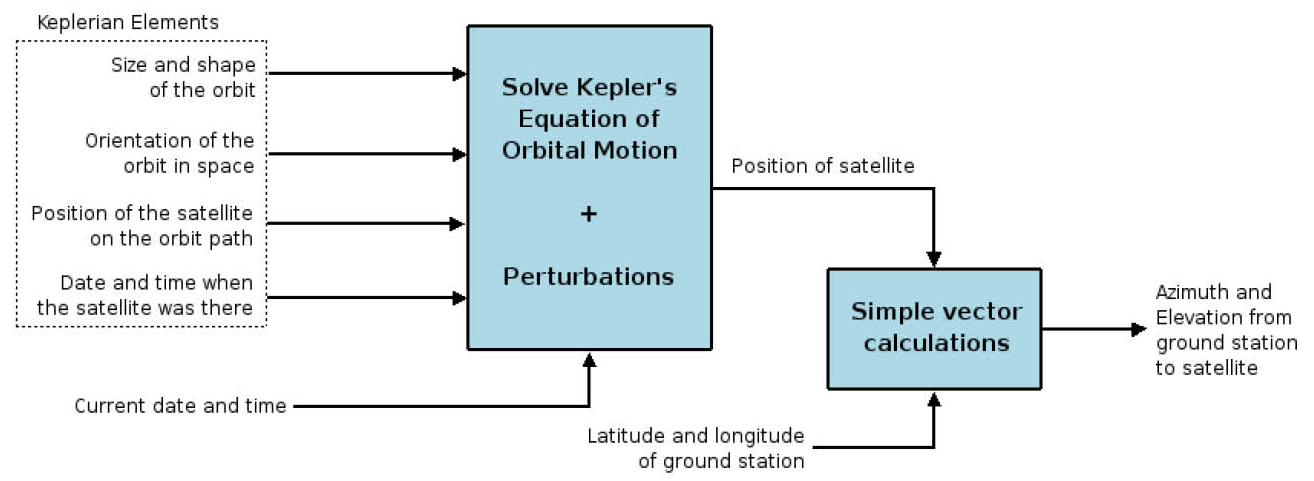
\includegraphics[width=1\textwidth]{gpredict-principle}
	\caption{Prinzip eines Satellitenverfolgungsprogramms, Quelle: \cite{gpredictmanual}}
	\label{fig:gpredict-principle} 
\end{figure}

\clearpage

Zur Berechnung der Satellitenposition wird auf den NORAD SGP4/SDP4 Algorithmus zurückgegriffen (siehe Abschnitt XXX). Um hierfür zu jedem Zeitpunkt die aktuellen Kepler-Elemente des zu verfolgenden Satelliten zu kennen, gibt es unter GPredict die Möglichkeit einer automatischen Aktualisierung über HTTP, FTP oder aus dem lokalen Verzeichnis.\newpar
Bei GPredict ist im Gegensatz zu anderen Satellitenverfolgungsprogrammen wie SatPC32 kein Limit an zu verfolgenden Satelliten und Bodenstationen gegeben. Durch die Verwendung von Modulen kann außerdem unkompliziert zwischen verschiedenen Konfigurationen gewechselt werden. Die Orbitvorhersage eines Satelliten lässt sich sowohl grafisch als auch tabellarisch darstellen, wobei durch die Einstellungen verschiedenster Parameter eine sehr individuelle Anzeige erreicht werden kann.

\section{Grafische Oberfläche}

In Abbildung \ref{fig:gpredictstartup} ist die grafische Oberfläche von GPredict zu sehen. In der Standardkonfiguration ist dort zunächst die Kartenansicht bzw. \myemph{Map View} (oben), die Polaransicht bwz. \myemph{Polar View} (links unten) und die Einzelsatellitenansicht bzw. \myemph{Single-Satellite View} (rechts unten) zu sehen.

\begin{figure}[h]
	\centering
	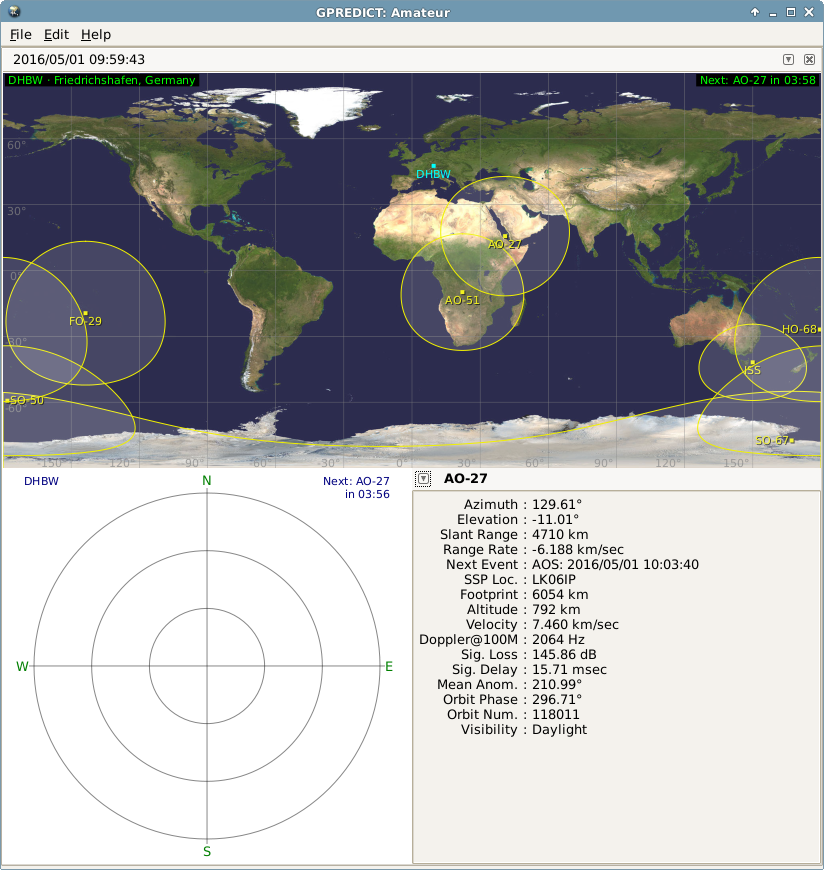
\includegraphics[width=0.54\textwidth]{gpredict-startup}
	\caption{Standardoberfläche von GPredict}
	\label{fig:gpredictstartup} 
\end{figure}

\clearpage

\subsection{Grundansichten}

Zu den oben genannten Ansichten kommen noch zwei Weitere hinzu, die Listenansicht bzw. \myemph{List View} und eine Ansicht für bevorstehende Durchläufe, die sogenannte \myemph{Upcoming Passes View}. Im Folgenden werden die verschiedenen Ansichten genauer beschrieben:\newpar
\textbf{Map View}\\
Diese Ansicht besteht, wie in Abbildung \ref{fig:gpredictstartup} zu sehen, aus einer Weltkarte auf der die aktuellen Standorte der für das aktuelle Modul ausgewählten Satelliten zu sehen ist. Das heißt der Punkt auf dem der entsprechende Satellit senkrecht bezogen auf den Erdmittelpunkt steht. Außerdem ist um diesen Punkt die Fläche umrahmt, von der der Satellit von der Erde aus sichtbar ist. Mit einem Rechtsklick auf einen Satellitennamen kann außerdem die Option \myemph{Ground Track} aktiviert werden, mit welcher die Spur des Satelliten für mehrere Orbits angezeigt wird.\newpar
\textbf{Polar View}\\
Die \myemph{Polar View} (siehe Abbildung \ref{fig:gpredictstartup}) stellt eine Draufsicht auf die Bodenstation dar, bei der die Polarachse den Azimutwinkel darstellt und die Radialachse den Elevationswinkel. Mit einem Rechtsklick auf einen Satelliten lässt sich mit der Option \myemph{Show sky track} aktivieren, das die Spur des entsprechenden Satelliten anzeigt wird. Zusätzlich wird das aktuelle Modul links oben angezeigt, der nächste sichtbare Satellit (rechts oben) und die genauen Werte für Azimut und Elevation (links unten) sobald sich der Mauszeiger auf der \myemph{Polar View} befindet.\newpar
\textbf{Single-Satellite View}\\
In dieser Ansicht (siehe Abbildung \ref{fig:gpredictstartup}) werden detaillierte Informationen zu einem ausgewählten Satelliten angezeigt, z.B. Azimut, Elevation, Entfernung der direkten Sichtverbindung (\myemph{Slant Range}), Höhe, Geschwindigkeit, Dopplerverschiebung oder Signaldämpfung. Mit einem Klick auf das \myvsymbol-Symbol links neben dem Satellitennamen kann zwischen den für dieses Modul ausgewählten Satelliten gewechselt werden.

\clearpage

\textbf{List View}\\
Die Listenansicht zeigt eine tabellarische Auflistung aller für das aktuelle Modul ausgewählten Satelliten mit verschiedenen Details, mit je einem Satelliten pro Zeile. In Abbildung \ref{fig:listview} ist die Listenansicht mit allen verfügbaren Details zu sehen. Mit einem Klick auf eine entsprechende Kategorie lässt sich das Sortierkriterium ändern. Falls hier ein variables Kriterium wie die Geschwindigkeit eingestellt wird, ändert sich die Sortierreihenfolge mit der eingestellten Auffrischrate (\myemph{Refresh Rate}). Die Bezeichnung des jeweiligen Details ist in dieser Ansicht abgekürzt, z.B. \myemph{Az} für \myemph{Azimut}. Unter den Moduleinstellungen beim Reiter \myemph{List View} kann ausgewählt werden, welches Detail angezeigt wird. Dort ist außerdem erkenntlich für was die entsprechenden Abkürzungen stehen.

\begin{figure}[h]
	\centering
	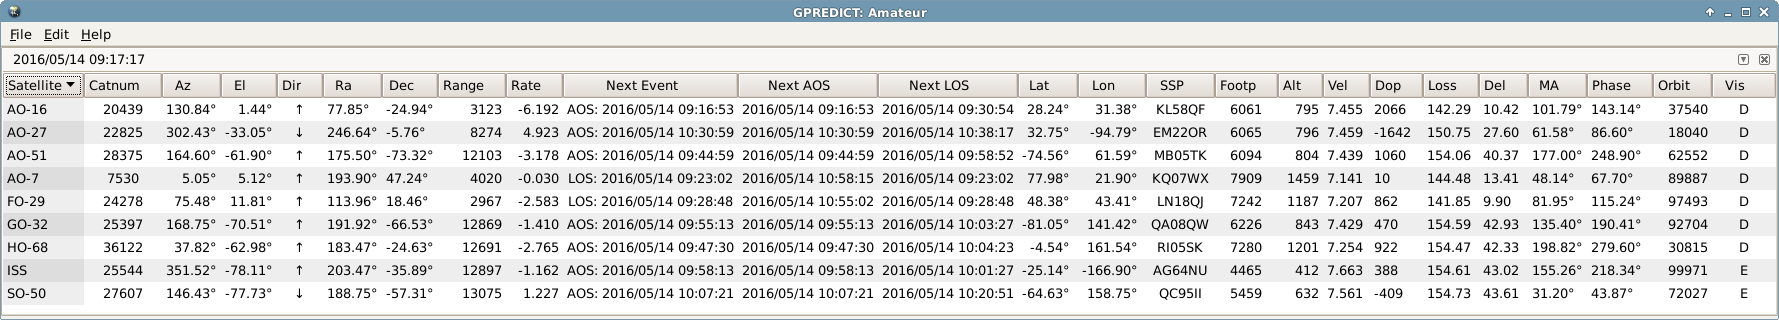
\includegraphics[width=1\textwidth]{listview}
	\caption{\myemph{List View}}
	\label{fig:listview} 
\end{figure}

\textbf{Upcoming Passes View}\\
Die \myemph{Upcoming Passes View} (siehe Abbildung \ref{fig:upcomingpassesview}) zeigt alle Satelliten des aktuellen Moduls, deren Azimut und Elevation, sowie die Zeit bis zum nächsten Verschwinden des Satelliten, dem sogenannten \myemph{\ac{LOS}} bzw. dem nächsten Auftauchen, auch \myemph{\ac{AOS}} genannt. Wie bei der \myemph{List View} ist es auch hier möglich nach den verschiedenen Spalten zu sortieren.

\begin{figure}[h]
	\centering
	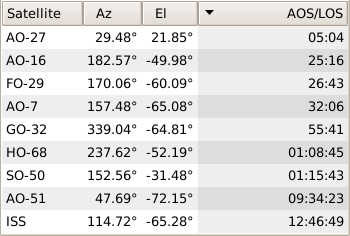
\includegraphics[width=0.4\textwidth]{upcomingpassesview}
	\caption{\myemph{Upcoming Passes View}}
	\label{fig:upcomingpassesview} 
\end{figure}

\clearpage

\subsection{Weitere Ansichten}

Bei allen Ansichten kann durch einen Klick auf den Satellitennamen ein kleines Pop-Up Menü geöffnet werden, welches den entsprechenden Satellitennamen, die Option \myemph{Show next pass} und die Option \myemph{Future passes} anzeigt. Bei einem Klick auf den Satellitennamen öffnet sich ein Fenster mit dem Titel \myemph{Satellite Info}, wie in Abbildung \ref{fig:satinfo} zu sehen. Dort sind unter dem Reiter \myemph{Orbit Info} verschiedene Informationen zum Satellitenorbit und unter dem Reiter \myemph{Transponders} die verfügbaren Transponder zu sehen.

% (bei der \myemph{Single-Satellite View} ein Klick auf das Dreieck neben dem Namen)
% (oder einen Doppelklick in der entsprechenden Ansicht auf den Satellitennamen)

\begin{figure}[h]
	\centering
	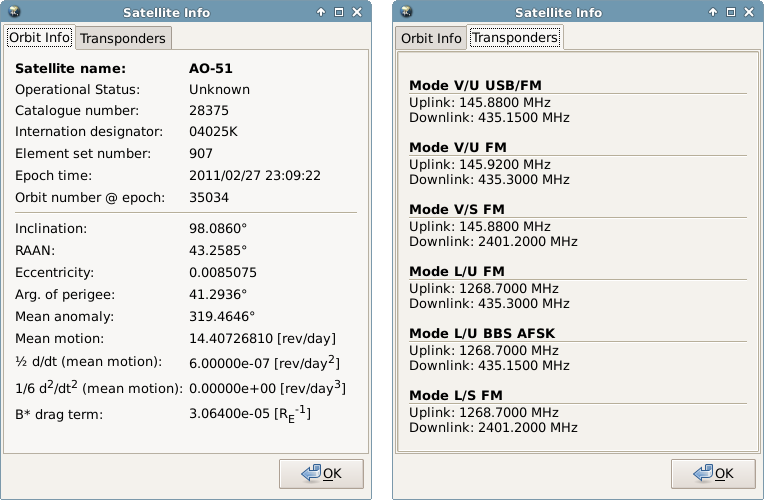
\includegraphics[width=0.65\textwidth]{satinfo}
	\caption{\myemph{Satellite Info}}
	\label{fig:satinfo} 
\end{figure}

Mit einem Klick auf die Option \myemph{Show next pass} gelangt man zu einer Übersicht über den nächsten Durchlauf des entsprechenden Satelliten. Die Details sind tabellarisch, als Polaransicht und als Verlauf des Azimut- und Elevationswinkels über der Zeit zu sehen (siehe Abbildung \ref{fig:passdetails}).

\begin{figure}[h]
	\centering
	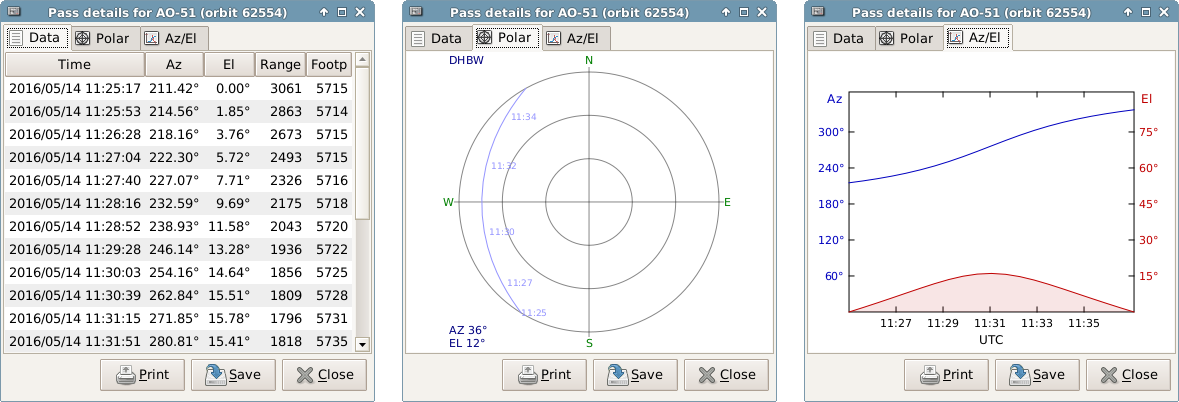
\includegraphics[width=1\textwidth]{passdetails}
	\caption{\myemph{Pass Details}}
	\label{fig:passdetails} 
\end{figure}

\clearpage

Die Option \myemph{Future passes} öffnet ein Fenster, in welchem die nächsten Durchläufe des entsprechenden Satelliten tabellarisch dargestellt sind (siehe Abbildung \ref{fig:upcomingpasses}). Hierbei ist die Anzahl der darzustellenden Durchläufe in den GPredict-Einstellungen unter \myemph{Predict} als \myemph{Number of passes to predict} einstellbar.

\begin{figure}[h]
	\centering
	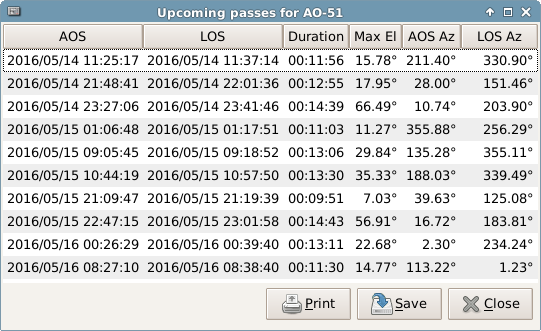
\includegraphics[width=0.5\textwidth]{upcomingpasses}
	\caption{\myemph{Upcoming Passes}}
	\label{fig:upcomingpasses} 
\end{figure}

\vspace{-0.5em}

\subsection{Modul Pop-Up Menü}

Um das Modul Pop-Up Menü zu öffnen, klickt man ganz rechts oben im GPredict-Fenster auf das \myvsymbol-Symbol. Im daraufhin erscheinenden Pop-Up Menü ist es möglich die Positionierung eines Moduls innerhalb des GPredict-Fensters einzustellen, ein Modul zu kopieren, zu löschen, zu schließen oder genauer zu konfigurieren. Außerdem sind dort weitere Funktionen, welche im Folgenden genauer beschrieben werden, zugänglich.\newpar
Wie in Abbildung \ref{fig:theskyataglance} zu sehen, bietet die Funktion \myemph{Sky at a glance} eine Übersicht darüber, wann welche Satelliten innerhalb der nächsten acht Stunden sichtbar sind. Dieser Zeitraum lässt sich in den GPredict-Einstellungen bei \myemph{Predict} unter dem Reiter \myemph{Sky at a Glance} zwischen einer und 24 Stunden einstellen.

\begin{figure}[h]
	\centering
	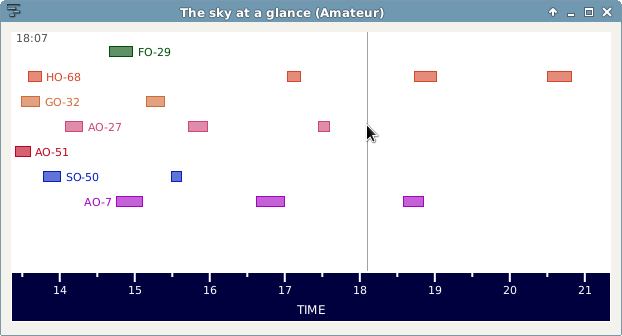
\includegraphics[width=0.5\textwidth]{theskyataglance}
	\caption{\myemph{The sky at a glance}}
	\label{fig:theskyataglance} 
\end{figure}

\clearpage

Über die Funktion \myemph{Time Controller} (siehe Abbildung \ref{fig:timecontroller}) lässt sich die Zeit, auf die sich die Berechnungen von GPredict beziehen, ändern. Hierbei ist standardmäßig das aktuelle Datum und die aktuelle Uhrzeit eingestellt. Außerdem kann hier die Geschwindigkeit, mit der die eingestellte Zeit fortschreitet, auf maximal ein Hundertfaches erhöht werden. Die eingestellte Zeit wird im GPredict-Fenster ganz links oben im ausgewählten Format angezeigt. Mit dem Schieberegler kann die Zeit zwischen --2,5 und +2,5 Stunden eingestellt werden.

\begin{figure}[h]
	\centering
	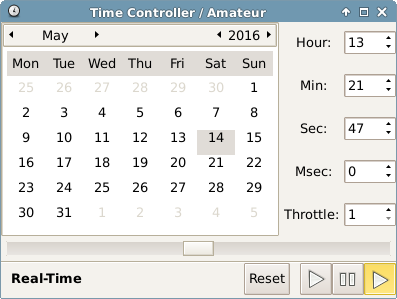
\includegraphics[width=0.35\textwidth]{timecontroller}
	\caption{\myemph{Time Controller}}
	\label{fig:timecontroller} 
\end{figure}

Klickt man auf \myemph{Configure}, öffnet sich ein Fenster wie in Abbildung \ref{fig:editmodule} zu sehen. Hier lassen sich die zu verfolgenden Satelliten und die Bodenstation für das aktuelle Modul auswählen. Außerdem gelangt man mit einem Klick auf das Feld \myemph{Properties} in die Modul-Einstellungen. Diese gelten im Gegensatz zu den in den allgemeinen GPredict-Einstellungen zu findenden Modul-Einstellungen nur für das aktuelle Modul. Auf Seite \pageref{modulesettingsgeneral} sind nähere Infos zu den Modul-Einstellungen zu finden.
\label{modulesettingsspecific}

\begin{figure}[h]
	\centering
	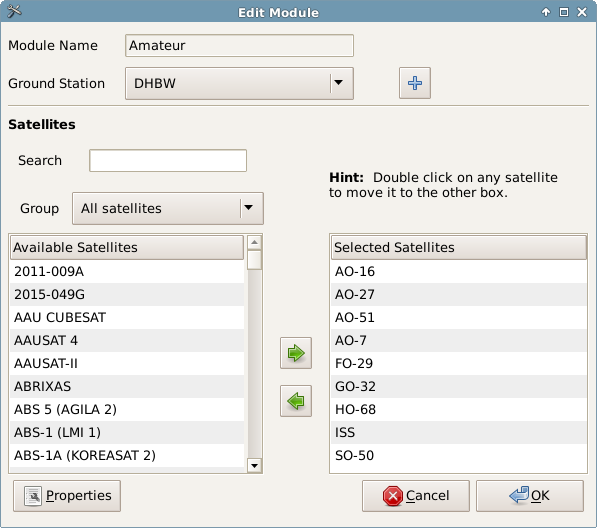
\includegraphics[width=0.5\textwidth]{editmodule}
	\caption{\myemph{Edit Module}}
	\label{fig:editmodule} 
\end{figure}

\clearpage

Hinter der Funktion \myemph{Antenna Control} (siehe Abbildung \ref{fig:rotatorcontrol}) verbirgt sich ein Bedienfeld zur Steuerung der Antennenrotoren. Bevor dieses geöffnet werden kann, muss zunächst in den GPredict-Einstellungen unter \myemph{Interfaces} mindestens eine Schnittstelle zur Rotorsteuerung konfiguriert werden (siehe Abschnitt XXX). 
\begin{figure}[h]
	\centering
	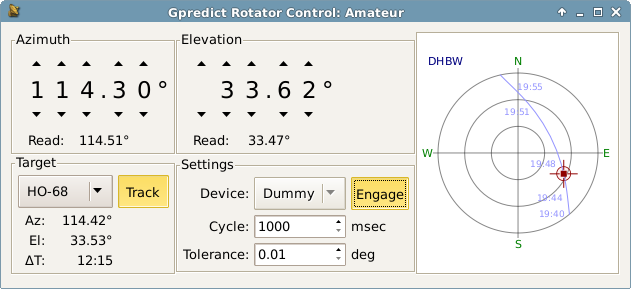
\includegraphics[width=0.6\textwidth]{rotatorcontrol-active}
	\caption{Rotorsteuerungs-Bedienfeld}
	\label{fig:rotatorcontrol} 
\end{figure}

Das Bedienfeld beinhaltet zum Einen eine Polaransicht, auf der die Spur und der aktuelle Ort des zu verfolgenden Satelliten (dargestellt durch ein Viereck) und die gegenwärtige Ausrichtung der Antenne (dargestellt durch ein Fadenkreuz) zu sehen ist. Zum Anderen sind folgende vier Bereiche verfügbar:

\begin{itemize}
	\parskip0pt
	\item \textbf{Azimuth:} In diesem Feld lässt sich die Ausrichtung der Antenne in Azimut-Richtung steuern, vorausgesetzt, dass die \myemph{Track}-Funktion nicht aktiviert ist. Am unteren Ende des Feldes wird unter \myemph{Read} der aktuelle Azimut-Winkel der Antenne angezeigt. Ist keine Verbindung zum Rotor aufgebaut, wird hier ,,-\,-\,-'' angezeigt. Liegt ein Verbindungsproblem vor, erscheint ,,ERROR''.
	\item \textbf{Elevation:} In diesem Feld lässt sich die Ausrichtung der Antenne in Elevations-Richtung steuern, vorausgesetzt, dass die \myemph{Track}-Funktion nicht aktiviert ist. Am unteren Ende des Feldes wird unter \myemph{Read} der aktuelle Elevations-Winkel der Antenne angezeigt. Ist keine Verbindung zum Rotor aufgebaut, wird hier ,,-\,-\,-'' angezeigt. Liegt ein Verbindungsproblem vor, erscheint ,,ERROR''.
	\item \textbf{Target:} Hier lässt sich der zu verfolgende Satellit auswählen. Es stehen hierbei nur die für das aktuelle Modul ausgewählten Satelliten zu Verfügung. Aktiviert man die Schaltfläche \myemph{Track}, wird der ausgewählte Satellit verfolgt. Unter dem Satellitennamen werden die jeweiligen Winkel in Echtzeit dargestellt und hinter $\Delta$T wird die Zeit bis zum nächsten \ac{AOS} bzw. \ac{LOS} angezeigt.
	\clearpage
	\item \textbf{Settings:} Hier lässt sich die in den GPredict-Einstellungen festgelegte Schnittstelle zur Kommunikation mit den Rotoren auswählen. Mit einem Klick auf die Schaltfläche \myemph{Engage} wird die Verbindung zu dieser Schnittstelle aufgebaut bzw. unterbrochen. Unter \myemph{Cycle} kann dabei der Zyklus eingestellt werden, in welchem Kommandos an die Rotor-Schnittstelle gesendet und Winkelwerte von dieser abgefragt werden. Ein sinnvoller Wert liegt hierbei zwischen zwei und fünf Sekunden. Bei \myemph{Tolerance} wird die tolerierte Differenz zwischen abgefragtem und eingestelltem Winkel eingetragen. Sobald diese überschritten wird, wird ein  Kommando an die Rotor-Schnittstelle geschickt. Hierbei sollte sowohl die Winkelauflösung der Rotorsteuerung, als auch die Keulenbreite der Antenne berücksichtigt werden. Nach fünf aufeinanderfolgenden Fehlern bei der Kommunikation mit den Rotoren, wird die Verbindung automatisch unterbrochen.
\end{itemize}

In Tabelle \ref{tab:rotatorcontrolmodes} sind alle möglichen Kombinationen der Schaltflächen \myemph{Track} und \myemph{Engage} und deren Auswirkung beschrieben.

\begin{table}[h]
	\begin{tabularx}{\textwidth}{|l|l|X|}
		\hline
		\textbf{Track} 	    & \textbf{Engage}	&\textbf{Beschreibung}\\
		\hline
		Inaktiv          	& Inaktiv 			& Es werden weder Kommandos an die Rotoren gesendet, noch wird die aktuelle Ausrichtung der Antenne ausgelesen. Die aktuellen Winkel des zu verfolgenden Satelliten werden nicht in die Winkelsteuerungs-Eingabefelder übertragen.\\
		Aktiv              	& Inaktiv   		& Die aktuellen Winkel des zu verfolgenden Satelliten werden in die Winkelsteuerungs-Eingabefelder übertragen, es werden aber keine Kommandos an die Rotoren geschickt und die aktuelle Ausrichtung der Antenne wird nicht ausgelesen.\\
		Aktiv              	& Aktiv	            & Die aktuellen Winkel des zu verfolgenden Satelliten werden in die Winkelsteuerungs-Eingabefelder übertragen und diese werden an die Rotoren geschickt. Die aktuelle Ausrichtung der Antenne wird ausgelesen.\\
		Inaktiv            	& Aktiv   			& Die Winkel, die in den Winkelsteuerungs-Eingabefelder eingestellt sind, werden an die Rotoren gesendet und die aktuelle Ausrichtung der Antenne wird ausgelesen.\\
		\hline		
	\end{tabularx}
	\caption{Betriebsmodi des \myemph{Antenna Control}-Bedienfelds, Quelle: \cite{gpredictmanual} \vspace{-2em}}
	\label{tab:rotatorcontrolmodes}
\end{table}

\clearpage

Um dem Funkgerät die entsprechenden Up- und Downlink-Frequenzen inklusive Dopplerschiftkorrektur zu übermitteln, wird das \myemph{Radio Control}-Bedienfeld (siehe Abbildung \ref{fig:radiocontrol}) verwendet. Dieses kann nur geöffnet werden, wenn mindestens eine Funkgerät-Schnittstelle in den GPredict-Einstellungen unter \myemph{Interfaces} konfiguriert ist (siehe Abschnitt XXX).

\begin{figure}[h]
	\centering
	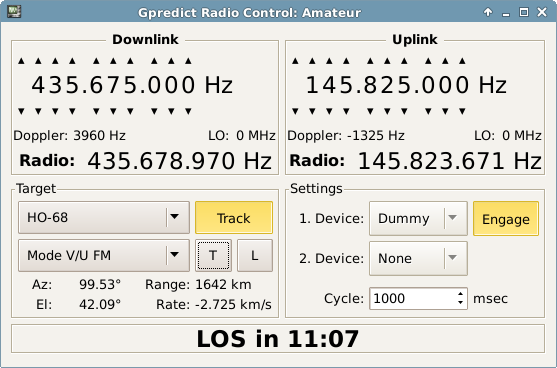
\includegraphics[width=0.6\textwidth]{radiocontrol-active}
	\caption{Funkgerät-Steuerung}
	\label{fig:radiocontrol} 
\end{figure}

Neben einer Anzeige die die Zeit bis zum nächsten \ac{AOS} bzw. \ac{LOS} darstellt (ganz unten im Bedienfeld in fettgedruckten Buchstaben) kann das \myemph{Radio Control}-Bedienfeld in folgende vier Bereiche untergliedert werden:

\begin{itemize}
	\parskip0pt
	\item \textbf{Downlink:} In diesem Bereich kann die Frequenzeinstellung für die Downlink-Frequenz vorgenommen werden. Außerdem ist die aktuelle Dopplerfrequenz und ein Feld names \myemph{LO}, welches für eine Offsetfrequenz steht, die im Funkgerät eingestellt werden kann, steht. Die korrigierte Frequenz welche nach \myemph{Radio} angezeigt wird, setzt sich damit beispielsweise wie folgt zusammen: $f_{Radio} = f_{Satellite} + f_{Doppler} - f_{LO}$
	\item \textbf{Uplink:} Dieser Bereich beinhaltet die Frequenzeinstellungen für die Uplink-Frequenz und besitzt die gleichen Eigenschaften wie der Downlink-Bereich.
	\item \textbf{Target:} Hier kann der zu verfolgende Satellit und der zu verwendente Transponder eingestellt werden. Mit einem Klick auf \myemph{Track} wird der Dopplerschift des ausgewählten Satelliten bei den Frequenzeinstellungen im Downlink- und Uplink-Bereich korrigiert. Eine wichtige Rolle spielt hierbei die Schaltfläche \myemph{T} (\myemph{Tune}), da die Frequenzen des Transponders nur durch einen Klick auf diese in die Frequenzeinstellungen übertragen werden. Sollte der Transponder beispielsweise nur einen Downlink besitzen, wird auch nur die Frequenz im Downlink-Bereich eingestellt.\clearpage
	Mit der Schaltfläche \myemph{L} (\myemph{Lock}) lässt sich die Differenz der Downlink- und Uplink-Frequenz sperren, das heißt Änderungen an der einen wirken sich auch auf die andere Frequenz aus. Dies ist nicht für Transponder möglich, die nur einen Up- oder Downlink besitzen.
	\item \textbf{Settings:} In diesem Bereich lassen sich bis zu zwei Funkgeräte auswählen die in den GPredict-Einstellungen unter \myemph{Interfaces} eingerichtet wurden. Das obere Gerät stellt das Primäre dar und kann für Up- und Downlink verwendet werden. Das Untere kann als sekundäres Gerät verwendet werden, welches nur für den Uplink verwendet werden kann. Mit einem Klick auf \myemph{Engage} wird die Kommunikation zwischen GPredict und Funkgerät(en) aufgebaut. Hierbei kann im Feld neben \myemph{Cycle} der Zyklus eingetragen werden, nach welchem Kommandos an das Funkgerät geschickt werden sollen.
\end{itemize}

In Tabelle \ref{tab:radiocontrolmodes} ist eine Übersicht über die verschiedenen Betriebsmodi des \myemph{Radio Control}-Bedienfelds zu sehen.

\begin{table}[h]
	\begin{tabularx}{\textwidth}{|l|l|X|}
		\hline
		\textbf{Track} 	    & \textbf{Engage}	&\textbf{Beschreibung}\\
		\hline
		Inaktiv          	& Inaktiv 			& Es wird keine Dopplerschiftkorrektur durchgeführt, keine Befehle an das Funkgerät gesendet und die aktuelle Frequenz des Funkgeräts nicht ausgelesen.\\
		Aktiv              	& Inaktiv   		& Die Dopplerschiftkorrektur wird durchgeführt, es werden aber weder Befehle an das Funkgerät geschickt noch wird die aktuelle Frequenz ausgelesen.\\
		Aktiv              	& Aktiv	            & Der Dopplerschift wird korrigiert und die eingestellte Frequenz wird zum Funkgerät geschickt. Die aktuelle Frequenz des Funkgeräts wird ausgelesen.\\
		Inaktiv            	& Aktiv   			& Die Dopplerschiftkorrektur wird nicht ausgeführt. Die eingestellte Frequenz wird an das Funkgerät geschickt und die dort eingestellte Frequenz wird ausgelesen.\\
		\hline		
	\end{tabularx}
	\caption{Betriebsmodi des \myemph{Radio Control}-Bedienfelds, Quelle: \cite{gpredictmanual}}
	\label{tab:radiocontrolmodes}
\end{table}

Wenn die \myemph{Engage}-Schaltfläche aktiviert ist, wird die Dopplerschiftkorrektur durchgeführt, egal ob der ausgewählte Satellit sichtbar ist oder nicht.

\clearpage

\subsection{GPredict-Einstellungen}

Um in die GPredict-Einstellungen zu gelangen, klickt man links oben unterhalb der Titelleiste auf \myemph{Edit} und anschließend auf \myemph{Preferences}. Nun öffnet sich ein Fenster bei dem standardmäßig die Erste der vier Kategorien zu sehen ist, die Kategorie \myemph{General} (siehe Abbildung \ref{fig:generalsettings}). Nach einer Veränderung in den GPredict-Einstellungen muss GPredict zunächst neugestartet werden, damit diese Änderung wirksam wird. Überall wo die Schaltfläche \myemph{Reset} zu finden ist, können mit einem Klick auf diese, die Standard-Einstellungen wiederhergestellt werden. Bei den meisten Optionen erscheint ein kleines Informations-Fenster, sobald man mit dem Mauszeiger einige Sekunden über der entsprechenden Option verharrt.

\begin{figure}[h]
	\centering
	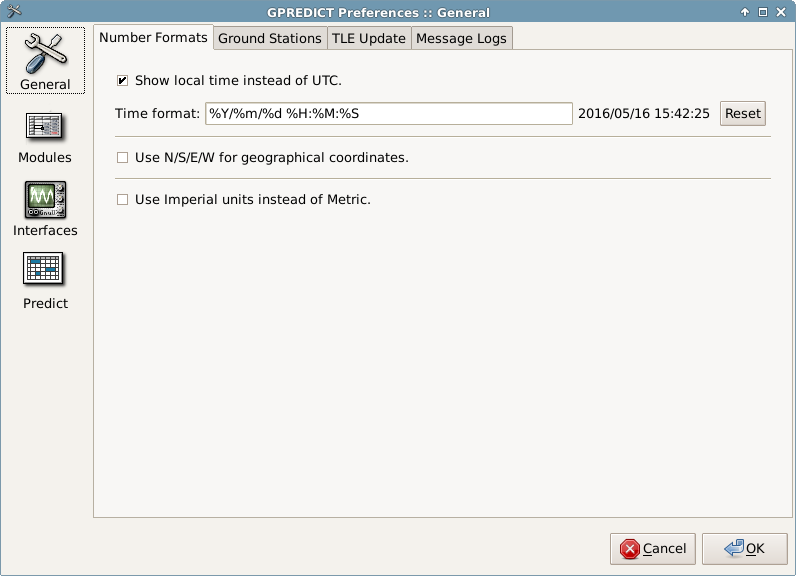
\includegraphics[width=0.65\textwidth]{generalsettings}
	\caption{GPredict-Einstellungen, Kategorie \myemph{General}}
	\label{fig:generalsettings} 
\end{figure}

Die Kategorie \myemph{General} ist in folgende vier Reiter untergliedert:

\begin{itemize}
	\parskip0pt
	\item \textbf{Number Formats:} Hier lassen sich Einstellungen zum Zeitformat, zu den geografischen Koordinaten und zu den Längen- und Geschwindigkeits-Einheiten vornehmen.
	\item \textbf{Ground Stations:} Unter diesem Reiter können beliebig viele Bodenstationen eingerichtet werden. Mindestens eine muss jedoch zu jeder Zeit vorhanden sein.
	\item \textbf{TLE Update:} Hier können Einstellungen zur Aktualisierung der Kepler-Elemente vorgenommen werden.
	\item \textbf{Message Logs:} Hier können Einstellungen bzgl. des GPredict-Protokolls vorgenommen werden. Unter \myemph{Log browser} im Menü \myemph{File} kann dieses dargestellt werden.
\end{itemize}

\clearpage

Zur Kategorie \myemph{Modules} gelangt man über zwei Wege. Der erste führt über die allgemeinen GPredict-Einstellungen, wie in diesem Abschnitt beschrieben. Der Zweite führt über das Modul Pop-Up Menü, wie auf Seite \pageref{modulesettingsspecific} beschrieben. Der Unterschied ist, dass bei den Modul-Einstellungen in den GPredict-Einstellungen die Standardwerte für alle Module eingestellt werden können und beim zweiten Weg nur die für das entsprechende Modul.
\label{modulesettingsgeneral}

%(siehe Abbildung \ref{fig:modulesettings})
\iffalse
\begin{figure}[h]
	\centering
	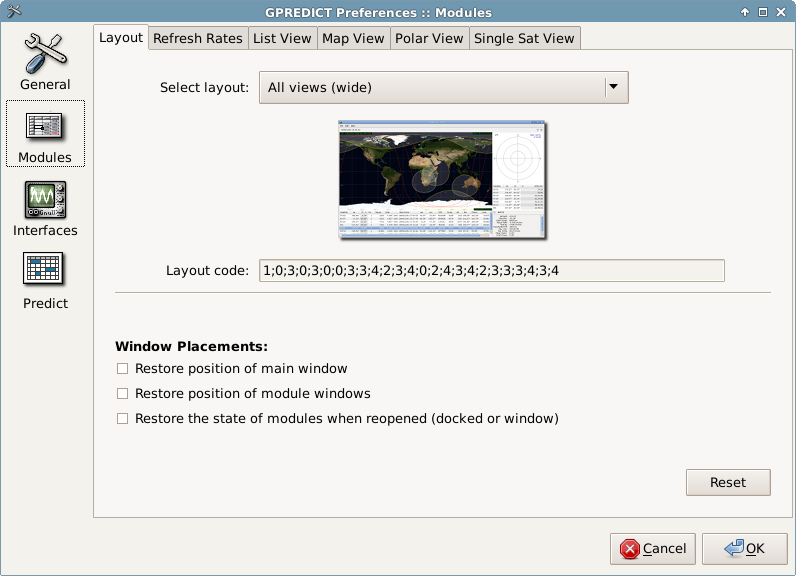
\includegraphics[width=0.65\textwidth]{modulesettings}
	\caption{GPredict-Einstellungen, Kategorie \myemph{Modules}}
	\label{fig:modulesettings} 
\end{figure}
\fi
Die Modul-Einstellungen sind in folgende sechs Reiter untergliedert:

\begin{itemize}
	\parskip0pt
	\item \textbf{Layout:} Bei diesem Reiter lässt sich konfigurieren, welche Ansichten in welcher Anordnung im GPredict-Fenster zu sehen sind. Hierbei kann aus verschiedenen Anordnungen ausgewählt werden oder eine völlig benutzerspezifische Anordnung erstellt werden (Hierfür wird an dieser Stelle auf \cite{gpredictmanual} Seite 67f verwiesen).
	\item \textbf{Refresh Rates:} Hier lässt sich die Zeitspanne auswählen, nach  welcher GPredict die Positions-Berechnungen periodisch für jeden Satelliten durchführt, der für das geöffnete Modul ausgewählt wurde. Außerdem lässt sich einstellen mit welchem ganzzahligem Vielfachen dieser Zeitspanne die einzelnen Ansichten aufgefrischt werden.
	\item \textbf{List View:} Hier lassen sich die Parameter der \myemph{List View} auswählen.
	\item \textbf{Map View:} Hier lassen sich Darstellungsoptionen für die \myemph{Map View} konfigurieren.
	\item \textbf{Polar View:} Hier lassen sich Darstellungsoptionen für die \myemph{Polar View} konfigurieren.
	\item \textbf{Single Sat View:} Hier lassen sich die Parameter der \myemph{Single Sat View} auswählen.
\end{itemize}

Die Kategorie \myemph{Interfaces} ist in zwei Reiter untergliedert, \myemph{Radios} und \myemph{Rotators}. Dort wird jeweils eine Liste der bereits eingerichteten Funkgeräte bzw. Rotoren angezeigt, welche standardmäßig leer ist. Die Anzahl der Geräte ist dabei nach oben nicht beschränkt. Die detaillierte Einrichtung ist in Abschnitt \ref{chap:configinterfaces} auf Seite \pageref{configinterfaces} genauer beschrieben.\newpar
Beim Öffnen der Kategorie \myemph{Predict} wird standardmäßig der Reiter \myemph{Pass Conditions} angezeigt. Unter diesem lassen sich folgende Parameter einstellen:

\begin{itemize}
	\parskip0pt
	\item \textbf{Minimum elevation:} Dieser Parameter gibt an, ab welcher Elevation von einem Durchlauf eines Satelliten ausgegangen wird. Das heißt, übersteigt die maximale Elevation diesen Wert, wird dieser Durchlauf in die \myemph{Upcoming Passes}, die \myemph{Pass Details} und die Ansicht \myemph{The sky at a glance} aufgenommen.
	\item \textbf{Number of passes to predict:} Anzahl der angezeigten zukünftigen Durchläufe.
	\item \textbf{Passes should occur within:} Dieser Parameter definiert den Zeitraum, in welchem zukünftige Durchläufe von GPredict berücksichtigt werden. So tritt entweder erst die Anzahl der angezeigten zukünftigen Durchläufe ein oder der Zeitraum in welchem zukünftige Durchläufe berücksichtigt werden sollen.
	\item \textbf{Time resolution:}	Hier kann die Zeitauflösung eingetragen werden, mit der der nächste Durchlauf in den \myemph{Pass Details} dargestellt wird. Je geringer die Auflösung, desto mehr Einträge werden angezeigt.
	\item \textbf{Number of entries:} Mit diesem Parameter kann die Anzahl der Eintrage des nächsten Durchlaufs in den \myemph{Pass Details} eingestellt werden. Hierbei ist zu beachten, dass diese Einstellung eine höhere Priorität als die Zeitauflösung besitzt.
	\item \textbf{Twilight threshold:} Dieser Parameter gibt an, ab welcher Elevation ein Satellit als sichtbar gilt. Für die Satellitenverfolgung spielt dieser Paramenter keine Rolle.
\end{itemize}

Unter den Reitern \myemph{Multiple Passes} und \myemph{Single Pass} lassen sich die Parameter auswählen, die in den Ansichten \myemph{Upcoming Passes} und \myemph{Pass Details} dargestellt werden, wohingegen beim Reiter \myemph{Sky at a Glance} Darstellungsoptionen für die Funktion \myemph{The sky at a glance} eingestellt werden können.\newpar
Eine detailliertere Beschreibung der GPredict-Einstellungen kann aus \cite{gpredictmanual} Seite 23ff entnommen werden.

\section{HamLib-Programmierschnittstelle}

\subsection{Übersicht}

Da es keinen einheitlichen Kommunikationsstandard für die zahlreichen Funkgeräte und Rotoren unterschiedlicher Hersteller gibt, ist für die Verwendung von GPredict eine applikationsspezifische Programmierschnittstelle oder auch \ac{API} erforderlich. Mit den \myemph{Ham Radio Control Libraries} (englisch für Amateurfunk-Kontrollbibliotheken), kurz HamLib, steht dem Benutzer eine solche \ac{API} zur Verfügung. HamLib ist unter der \ac{GPL} lizenziert und ist unter \cite{hamlibdownload} in der Version 3.0.1 als Download für Linux und Windows kostenlos verfügbar. Wie in Abbildung \ref{fig:hamlib} zu sehen, ermöglicht HamLib einer Software wie GPredict die Kommunikation mit verschiedenen Funkgeräten und Rotoren, in dem es für jedes dieser Geräte einen eigenen Treiber bzw. ein eigenes \ac{BE} zur Verfügung stellt.

\begin{figure}[h]
	\centering
	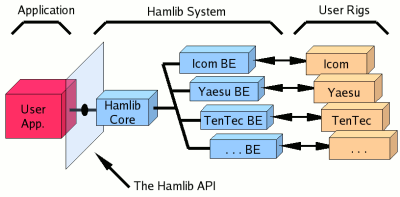
\includegraphics[width=0.5\textwidth]{hamlib}
	\caption{HamLib Design, Quelle: \cite{hamlibmanual}}
	\label{fig:hamlib} 
\end{figure}

Dabei verwendet man entweder den Quellcode um eine benutzerspezifische Anwendung zu erstellen oder man greift auf die bereits fertig kompilierten Programme zurück, welche im Folgenden aufgelistet sind:

\begin{itemize}
	\parskip0pt
	\item \textbf{rigctl:} Ein Kommandozeilenprogramm, mit welchem man Befehle über die Kommandozeile an das Funkgerät senden kann. (Unter Windows: \myemph{rigctl.exe})
	\item \textbf{rotctl:} Ein Kommandozeilenprogramm, mit welchem man Befehle über die Kommandozeile an die Antennenrotoren senden kann. (Unter Windows: \myemph{rotctl.exe})
	\item \textbf{rigctld:} Ein Kommandozeilenprogramm, mit welchem man Befehle über das TCP/IP-Protokoll an das Funkgerät senden kann (Unter Windows: \myemph{rigctld.exe})
	\item \textbf{rotctld:}  Ein Kommandozeilenprogramm, mit welchem man Befehle über das TCP/IP-Protokoll an die Antennenrotoren senden kann (Unter Windows: \myemph{rigctld.exe})
\end{itemize}

Hierbei steht ,,\myemph{rot}'' für ,,Rotator'' (deutsch: Rotor), ,,\myemph{rig}'' für  ,,Rig'' (deutsch: Amateurfunkgerät) und das ,,\myemph{d} am Ende von \myemph{rigctld} und \myemph{rotctld} für ,,Deamon'' (deutsch: Hintergrundprozess).



\subsection{Parameter-Konfiguration}
\label{chap:hamlibconfig}

Für die erfolgreiche Nutzung der oben genannten Programme müssen einige Optionen und Parameter berücksichtigt werden. Hierfür ist es notwendig die erforderlichen Informationen zu den Rotoren und zum Funkgerät zu kennen. Um eine Übersicht der möglichen Optionen und Befehle zu erhalten, kann das jeweilige Programm einfach mit der Option \texttt{-h} oder \texttt{-\,-help} ausgeführt werden.

\clearpage

Die erste zentrale Information ist die \myemph{Hamlib ID}. Hierfür gibt man folgenden Befehl in die Kommandozeile ein und erhält eine Liste mit allen unterstützten Funkgeräten (für \myemph{rigctld.exe} und \myemph{rotctl(d).exe} analog durchführbar):

\vspace{-1em}
\begin{shaded}
	\texttt{rigctl.exe -l}
\end{shaded}
\vspace{-1em}

Im Folgenden sind die beiden Zeilen dargestellt, die für die in diesem Projekt verwendeten Funkgerät und Rotoren relevant sind. Hierbei steht der erste Eintrag für die \myemph{Hamlib ID}, der Zweite für den Hersteller, der Dritte für die Version und der Vierte für den Test-Status:

\vspace{-1em}
\begin{shaded}
	\texttt{368\qquad Icom\qquad\ IC-9100\qquad 0.7\qquad Untested}\\%[-0.5em]
	\texttt{601\qquad Yaesu\qquad GS-232A\qquad 0.3\qquad Beta}
\end{shaded}
\vspace{-1em}

Als Nächstes muss die Schnittstelle zum Funkgerät bzw. zur Rotorensteuerung angegeben werden. Bei der im Rahmen diesen Projekts verwendeten Software (siehe Abschnitt \ref{chap:software}) werden hierfür serielle Schnittstellen verwendet. Wie diese konfiguriert werden, ist im folgenden Auszug aus der Hilfe, die bei Eingabe der Option \texttt{-h} oder \texttt{-\,-help} erscheint (für \myemph{rigctl.exe}), zu sehen:

\vspace{-1em}
\begin{shaded}
	 \texttt{-r, --rig-file=DEVICE\qquad \qquad select radio model number. See model list} \\%[-0.5em]
	 \texttt{-s, --serial-speed=BAUD\qquad\quad set serial speed of the serial port} \\%[-0.5em]
	 \texttt{-C, --set-conf=PARM=VAL\qquad \quad set config parameters}
\end{shaded}
\vspace{-1em}

Um eine Liste der gültigen Konfigurationsparameter (\texttt{config parameters}) auszugeben, führt man \myemph{rigctl(d).exe} bzw. \myemph{rotctl(d).exe} mit der Option \texttt{-L} oder \texttt{-\,-show-conf} aus. Die genauen Werte sind in Abschnitt \ref{chap:software} aufgeführt.\newpar
Im Testbetrieb ist die Ausgabe von Statusmeldungen (z.B. Warnungen oder Fehler) oft sehr hilfreich. Hierfür lässt sich mit der Option \texttt{-v} die Intensität der Ausgabe einstellen. Bei \texttt{-v} werden nur grobe Fehler ausgegeben, wohingegen bei \texttt{-vvvvv} alle verfügbaren Statusmeldungen der \ac{API} ausgegeben werden. Bei Weglassen der Option erfolgt keine Ausgabe. Mit diesem Wissen sieht die Ausführung des Programms \myemph{rotctl.exe} im Rahmen dieses Projekts wie folgt aus:

\vspace{-1em}
\begin{shaded}
	\texttt{rotctl.exe -vvvv -m 601 -r COM10 -s 9600 -C stop\_bits=1,data\_bits=8}
\end{shaded}
\vspace{-1em}

\clearpage

Da beim Funkgerät IC-9100 das Icom-spezifische Protokoll \acsu{CI-V} (das ,,V'' steht hierbei für die römische Zahl) für die Fernsteuerung verwendet wird, kommt bei der Verwendung von \myemph{rigctl.exe} noch die CI-V-Adresse als Parameter hinzu. Somit sieht die Ausführung des Programms \myemph{rigctl.exe} wie folgt aus: 

\vspace{-1em}
\begin{shaded}
	\small{\texttt{rigctl.exe -vvvv -m 368 -r COM5 -c 0x7C -s 19200 -C stop\_bits=1,data\_bits=8}}
\end{shaded}
\vspace{-1em}

\subsection{Verwendung}

Nachdem das Programm \myemph{rigctl.exe} bzw. \myemph{rotctl.exe} mit den unter Abschnitt \ref{chap:hamlibconfig} dargestellten Parametern gestartet wurde, hat man die Möglichkeit Befehle an das Funkgerät bzw. an die Rotorsteuerung zu senden.\newpar
\textbf{Beschreibung der folgenden Funktion}

\vspace{-1em}
\begin{shaded}
	\texttt{rigctl.exe -m 368 -u}\\
	\texttt{rotctl.exe -m 601 -u}
\end{shaded}
\vspace{-1em}

\textbf{Folgenden Text umschreiben}

Um die Verwendung dieser Kommandozeilenprogramme zu vereinfachen und um gleichzeitig die notwendige Konfiguration festzuhalten, wurde für die Programme \myemph{rigctl}, \myemph{rigctld}, \myemph{rotctl} und \myemph{rotctld} jeweils ein Batch-Skript erstellt (siehe Anhang \ref{chap:rigctldbat}, \ref{chap:rotctldbat}, XXX und YYY). Bei der Verwendung unter Linux können diese ohne Umstände in Bash-Skripte umgeschrieben werden. Diese Skripte müssen beide gestartet werden, bevor unter GPredict eine Kommunikation mit den Rotoren bzw. mit dem Funkgerät stattfinden kann.

\section{Inbetriebnahme unter Windows}

\subsection{Zusätzliche Software}
\label{chap:software}

\textbf{Blockschaltbild von (Hard- und) Softwarekomponenten}

\clearpage

\subsection{Konfiguration der Rotoren}
\label{chap:configinterfaces} \label{configinterfaces}

\textbf{GPredict kann auch von anderem PC ausgeführt werden und über das Netzwerk mit HamLib kommunizieren \-> Einstellung der IP-Adresse und des Ports}	

\vspace{-1em}
\begin{shaded}
	\texttt{rotctld.exe -T 127.0.0.1 -t 4533 \&}
\end{shaded}
\vspace{-1em}

\subsection{Konfiguration des Funkgeräts}

\textbf{GPredict kann auch von anderem PC ausgeführt werden und über das Netzwerk mit HamLib kommunizieren \-> Einstellung der IP-Adresse und des Ports}

\vspace{-1em}
\begin{shaded}
	\texttt{rigctld.exe -T 127.0.0.1 -t 4532 \&}
\end{shaded}
\vspace{-1em}

\subsection{Test der Kommunikation}

Parameter \texttt{post\_write\_delay} etc. erwähnen.\newpar

Test einiger Befehle mit \myemph{rigctl} und \myemph{rotctl}. 

\begin{itemize}
	\parskip0pt
	\item Auslesen und Setzen der Frequenz
	\item Auslesen und Setzen des Winkels
\end{itemize}

$\rightarrow$ \myemph{rigctl} und \myemph{rotctl} Skripte in Anhang einfügen!

\subsection{Test der Bedienfelder}

Test mit Dummy-Interfaces. $\rightarrow$ Hinweis auf Dummy-Skripte

\subsection{Finaler Test}

% \section{Inbetriebnahme unter Linux}